\documentclass{article}
\usepackage{amsthm,amsmath,amsfonts,lipsum}
\usepackage[T1]{fontenc}
\usepackage{beramono}
\usepackage{listings}
\usepackage{fontawesome5}
\usepackage{adjustbox}
\usepackage{mathabx}
\usepackage{thmtools}
\usepackage{import}
\usepackage{graphicx}
\usepackage{setspace}
\usepackage{geometry}
\usepackage{physics}
\usepackage{float}
\usepackage[english]{babel}
\usepackage{framed}
\usepackage[dvipsnames,x11names]{xcolor}
\usepackage{tcolorbox}
\usepackage{fancyhdr}
\usepackage{hyperref}
\usepackage{booktabs}
\usepackage{enumitem}
\usepackage{cancel}
\usepackage{background}
\usepackage{units}
\usepackage{textcomp}

% Configuring the background
\backgroundsetup{
  scale=1, % Optional, scale if needed
  color=black, % Optional, set the image color, can be omitted
  opacity=0.18, % Optional, adjust opacity for watermark effect
  angle=0,
  position=current page.center, % Center the image on the page
  contents={
\includegraphics[width=1.75\paperwidth, height=1.75\paperheight, keepaspectratio]{ninym_ralei_leaf (watermarked by AlexanderTheMango)}} % Keeps aspect ratio and scales to fill the page
}

% Colours
\definecolor{darkgreen}{rgb}{0.0, 0.5, 0.0}
\definecolor{Firebrick}{rgb}{0.698, 0.132, 0.203}
\definecolor{Crimson}{rgb}{0.862745, 0.078431, 0.235294} % Crimson color
\definecolor{lightred}{rgb}{1.0, 0.819608, 0.819608} % Light red for background
\definecolor{MediumPurple}{rgb}{0.576, 0.439, 0.859}
\definecolor{chocolate}{rgb}{0.82, 0.41, 0.12} % Chocolate color definition
\definecolor{myframecolor}{rgb}{0.25, 0.41, 0.88} % RoyalBlue
\definecolor{mybackgroundcolor}{rgb}{0.68, 0.85, 0.90} % LightSkyBlue
% Define the Navy color
\definecolor{Navy}{rgb}{0.0, 0.0, 0.5}

% Define custom tcolorbox styles for notes
\tcbuselibrary{skins, breakable}
\newtcolorbox{definitionbox}{colframe=RoyalBlue, colback=blue!5!white, title=Definition}
\newtcolorbox{examplebox}{colframe=ForestGreen, colback=green!5!white, title=Example}
\newtcolorbox{notebox}{colframe=RedOrange, colback=orange!5!white, title=Note}
\newtcolorbox{theorembox}{colframe=RoyalPurple, colback=purple!5!white, title=Theorem}

\newtcolorbox{propositionbox}{colframe=myframecolor, colback=mybackgroundcolor!20!white, title=Proposition}
\newtcolorbox{remarkbox}{colframe=MidnightBlue, colback=blue!10!white, title=Remark}
\newtcolorbox{corollarybox}{colframe=OliveGreen, colback=green!10!white, title=Corollary}
\newtcolorbox{warningbox}{colframe=Crimson, colback=lightred, title=Warning}
\newtcolorbox{proofbox}{colframe=Black, colback=gray!10!white, title=Proof}
\newtcolorbox{questionbox}{colframe=Teal, colback=teal!10!white, title=Question}
\newtcolorbox{tipbox}{colframe=Goldenrod, colback=yellow!10!white, title=Tip}
\newtcolorbox{exercisebox}{colframe=darkgreen, colback=green!5!white, title=Exercise}
\newtcolorbox{solutionbox}{colframe=DodgerBlue4, colback=blue!5!white, title=Solution}
\newtcolorbox{algorithmbox}{colframe=Navy, colback=blue!10!white, title=Algorithm}
\newtcolorbox{conceptbox}{colframe=chocolate, colback=brown!10!white, title=Concept}
\newtcolorbox{illustrationbox}{colframe=Firebrick, colback=red!10!white, title=Illustration}
\newtcolorbox{intuitionbox}{colframe=MediumPurple, colback=purple!10!white, title=Intuition}
\newtcolorbox{answerbox}{colframe=RoyalBlue, colback=blue!10!white, title=Answer}

% Geometry settings
\geometry{letterpaper, portrait, includeheadfoot=true, hmargin=1in, vmargin=1in}
\onehalfspacing

% Header and footer
\pagestyle{fancy}
\fancyhf{}
\lhead{MAT232 - Lecture Notes}
\rhead{\thepage}
\lfoot{University of Toronto Mississauga}
\rfoot{\today}

% Document starts
\begin{document}
\renewcommand{\familydefault}{\rmdefault}

\begin{titlepage}
    \null % This is a TeX command that does nothing but is necessary for vfill to work correctly
    \vfill
    \begin{center}
        {\fontsize{40}{48}\selectfont \bfseries MAT232 - Lecture 13}
        \vspace{20pt} \\
        {\LARGE after partial derivatives?} \\
        \vspace{20pt}
        \textbf{AlexanderTheMango}
        \vspace{8pt}
        \\ Prepared for February 24, 2025
    \end{center}
    \vfill
\end{titlepage}

\addcontentsline{toc}{section}{Title Page}

\newpage
\setcounter{page}{0}
\tableofcontents
\addcontentsline{toc}{section}{Table of Contents}
\newpage

\begin{titlepage}
    \null % Ensures proper alignment with vfill
    \vfill
    \begin{center}
        {\Huge \textbf{Definitions and Theorems}} \\[20pt]
        \rule{\textwidth}{0.5mm} \\[15pt]
        {\Large \textit{Straight from the textbook — lots of fluff this time, more than what we need!}} \\[15pt]
        \rule{\textwidth}{0.5mm} \\[15pt]
        \textbf{Quick recap before diving into the lecture.}
    \end{center}
    \vfill
\end{titlepage}


\section*{Polar Coordinates - Key Theorems}
\addcontentsline{toc}{section}{Polar Coordinates - Key Theorems}

\subsection*{Converting Points between Coordinate Systems}
\addcontentsline{toc}{subsection}{Converting Points between Coordinate Systems}
\begin{theorembox}
    Given a point \( P \) in the plane with Cartesian coordinates \( (x,y) \) and polar coordinates \( (r,\theta) \), the following conversion formulas hold true:
    \[
    x = r \cos\theta \quad \text{and} \quad y = r \sin\theta,
    \]
    \[
    r^2 = x^2 + y^2 \quad \text{and} \quad \tan\theta = \frac{y}{x}.
    \]
    These formulas can be used to convert between rectangular and polar coordinates.
\end{theorembox}

\subsection*{Uniqueness of Polar Coordinates}
\addcontentsline{toc}{subsection}{Uniqueness of Polar Coordinates}
\begin{propositionbox}
    Every point in the plane has an infinite number of representations in polar coordinates. Specifically, the polar coordinates \( (r, \theta) \) of a point are not unique.
    
    \begin{remarkbox}
        For example, the polar coordinates \( (2, \pi/3) \) and \( (2, 7\pi/3) \) both represent the same point in the rectangular coordinate system. Additionally, the value of \( r \) can be negative. Therefore, the point with polar coordinates \( (-2, 4\pi/3) \) represents the same rectangular point as \( (2, \pi/3) \).
    \end{remarkbox}
\end{propositionbox}

\subsection*{Symmetry of Polar Curves}
\addcontentsline{toc}{subsection}{Symmetry of Polar Curves}
\begin{theorembox}
    Polar curves can exhibit symmetry similar to those in rectangular coordinates. The key symmetries to identify are:
    \begin{itemize}
        \item \textbf{Symmetry with respect to the polar axis:} A curve is symmetric with respect to the polar axis if replacing \( \theta \) with \( -\theta \) in its equation yields the same curve.
        \item \textbf{Symmetry with respect to the line \( \theta = \frac{\pi}{2} \):} A curve is symmetric with respect to the line \( \theta = \frac{\pi}{2} \) if replacing \( \theta \) with \( \pi - \theta \) yields the same curve.
        \item \textbf{Symmetry with respect to the pole (origin):} A curve is symmetric with respect to the pole if replacing \( r \) with \( -r \) yields the same curve.
    \end{itemize}
\end{theorembox}

\begin{titlepage}
    \null % Ensures proper alignment with vfill
    \vfill
    \begin{center}
        {\Huge \textbf{Let’s Get Started}} \\[20pt]
        \rule{\textwidth}{0.5mm} \\[15pt]
        {\Large \textit{Time to dive into the lecture notes.}} \\[15pt]
        \rule{\textwidth}{0.5mm} \\[15pt]
        \textbf{Grab your pen or pencil, and let’s break this down step by step.}
    \end{center}
    \vfill
\end{titlepage}

\setcounter{page}{2}
\normalsize

\section*{Plotting Polar Coordinates}
\addcontentsline{toc}{section}{Plotting Polar Coordinates}

\subsection*{Recall the Content from Last Lecture}
\addcontentsline{toc}{subsection}{Recall the Content from Last Lecture}
\begin{notebox}
Converting between Cartesian coordinates \( (x, y) \) and Polar coordinates \( (r, \theta) \):

\begin{algorithmbox}
    \textbf{From Cartesian to Polar:}
    \[
        r = \sqrt{x^2 + y^2}, \quad \theta = \arctan\left(\frac{y}{x}\right)
    \]
    
    \textbf{From Polar to Cartesian:}
    \[
        x = r\cos\theta, \quad y = r\sin\theta
    \]
\end{algorithmbox}

\textbf{Converting Between Degrees and Radians:}
\begin{algorithmbox}
    \begin{itemize}
        \item \textbf{Degrees to Radians:} Multiply by \( \dfrac{\pi}{180^{\circ}} \)
        \[
        \text{Radians} = \text{Degrees} \times \dfrac{\pi}{180^\circ}
        \]
        \item \textbf{Radians to Degrees:} Multiply by \( \dfrac{180^\circ}{\pi} \)
        \[
        \text{Degrees} = \text{Radians} \times \dfrac{180^\circ}{\pi}
        \]
    \end{itemize}
\end{algorithmbox}
\end{notebox}

\subsection*{Understanding the Convention for \( r \) in Polar Coordinates}
\addcontentsline{toc}{subsection}{Understanding the Convention for \( r \) in Polar Coordinates}

\begin{conceptbox}
In polar coordinates, a \textbf{point} is represented as \( (r, \theta) \), where:
\begin{itemize}
    \item \( r \) is the radial distance from the origin (how far the point is from the origin).
    \item \( \theta \) is the angle, measured counterclockwise from the positive x-axis.
\end{itemize}

\begin{notebox}
    \subsubsection*{Special Case: When \( r \) is Negative}
    \begin{itemize}
        \item A negative \( r \) in \( (-r, \theta) \) is interpreted as the point being reflected through the origin.
        \item The equivalent representation is:
        \[
        (-r, \theta) = (r, \theta + 180^\circ)
        \]
        or in radians:
        \[
        (-r, \theta) = (r, \theta + \pi)
        \]
    \end{itemize}
\end{notebox}

\begin{intuitionbox}
    \begin{itemize}
        \item Reflecting \( (r, \theta) \) through the origin is the same as rotating the point by \( 180^\circ \) (or \( \pi \) radians).
        \item This property simplifies polar plots by offering alternate representations of the same point.
    \end{itemize}
\end{intuitionbox}
\end{conceptbox}

\begin{tipbox}
    When plotting points, ensure to label points clearly on the polar grid, and verify angle conversions and reflections for accuracy.
\end{tipbox}

\subsection*{Example: Plotting Points}
\addcontentsline{toc}{subsection}{Example: Plotting Points}

\begin{examplebox}
Let us plot the following points in polar coordinates:
\[
(3, -45^\circ), \quad (3, 225^\circ), \quad (4, 330^\circ), \quad (1, -45^\circ)
\]

\begin{algorithmbox}
    \textbf{Step-by-Step Process:}
    \begin{enumerate}
        \item For each point, identify \( r \) and \( \theta \).
        \item If \( \theta \) is negative or exceeds \( 360^\circ \), convert it to a standard range:
        \[
        \theta \in [0^\circ, 360^\circ)
        \]
        using \( \theta = \theta + 360^\circ \) (for negative angles) or subtracting \( 360^\circ \) (for angles over \( 360^\circ \)).
        \item Plot the point by measuring \( \theta \) counterclockwise from the positive x-axis and placing it at a distance \( r \) from the origin.
    \end{enumerate}
\end{algorithmbox}

\begin{solutionbox}
    \begin{itemize}
        \item For \( (3, -45^\circ) \): Add \( 360^\circ \) to \(-45^\circ\) to convert \( \theta \) to \( 315^\circ \). Plot as \( (3, 315^\circ) \).
        \item For \( (3, 225^\circ) \): Already within the standard range, so plot directly.
        \item For \( (4, 330^\circ) \): Angle is standard, so plot directly.
        \item For \( (1, -45^\circ) \): Add \( 360^\circ \) to \(-45^\circ\), yielding \( (1, 315^\circ) \).
    \end{itemize}
    
    \begin{figure}[H]
        \centering
        \begin{minipage}{0.3\textwidth}
            \centering
            
\includegraphics[width=\textwidth]{plot points.png}
            \caption{Colour Legend}
            \label{fig:image1}
        \end{minipage}%
        \hspace{0.04\textwidth} % Adds horizontal space between the images
        \begin{minipage}{0.65\textwidth}
            \centering
            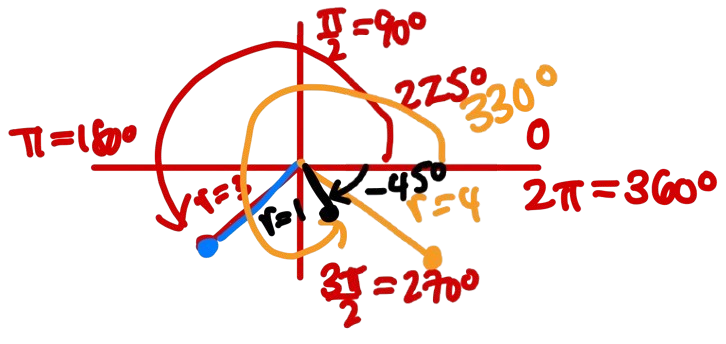
\includegraphics[width=\textwidth]{plot points example.png}
            \caption{Polar Coordinates Plot and ``Trajectories''}
            \label{fig:image2}
        \end{minipage}
    \end{figure}    
\end{solutionbox}
\end{examplebox}

\section*{Converting Between Cartesian and Polar Coordinates}
\addcontentsline{toc}{section}{Converting Between Cartesian and Polar Coordinates}

\subsection*{Example: Converting from Polar Coordinates to Cartesian Coordinates}
\addcontentsline{toc}{subsection}{Example: Converting from Polar Coordinates to Cartesian Coordinates}

\begin{examplebox}
Find the \textbf{rectangular coordinates} of the point \( p \) with polar coordinates \( (6, \dfrac{\pi}{3}) \).

\begin{solutionbox}
To convert from polar to Cartesian coordinates, use:
\[
    x = r \cos \theta, \quad y = r \sin \theta
\]

Substitute \( r = 6 \) and \( \theta = \frac{\pi}{3} \):
\[
    x = 6 \cos\left(\frac{\pi}{3}\right) = 6 \cdot \frac{1}{2} = 3, \quad
    y = 6 \sin\left(\frac{\pi}{3}\right) = 6 \cdot \frac{\sqrt{3}}{2} = 3\sqrt{3}.
\]

Thus, the Cartesian coordinates are:
\[
    (x, y) = (3, 3\sqrt{3}).
\]

\begin{answerbox}
The rectangular coordinates are \( (3, 3\sqrt{3}) \).
\end{answerbox}
\end{solutionbox}
\end{examplebox}

\subsection*{Example: Converting from Cartesian Coordinates to Polar Coordinates}
\addcontentsline{toc}{subsection}{Example: Converting from Cartesian Coordinates to Polar Coordinates}
\begin{examplebox}
Find the \textbf{polar coordinates} of the point \( p \) with rectangular coordinates \( (-2, 2\sqrt{3}) \).

\begin{solutionbox}
To find the polar coordinates, use:
\[
    r^2 = x^2 + y^2, \quad \tan(\theta) = \frac{y}{x}.
\]

\textbf{Step 1: Solve for \( r \):}
\[
    r^2 = (-2)^2 + (2\sqrt{3})^2 = 4 + 12 = 16 \implies r = 4.
\]

\textbf{Step 2: Solve for \( \theta \):}
\[
    \tan(\theta) = \frac{y}{x} = \frac{2\sqrt{3}}{-2} = -\sqrt{3}.
\]

The point \( (-2, 2\sqrt{3}) \) lies in Quadrant II. The reference angle for \( \tan^{-1}(\sqrt{3}) \) is \( \frac{\pi}{3} \). Thus:
\[
    \theta = \pi - \frac{\pi}{3} = \frac{2\pi}{3}.
\]

\begin{tipbox}
    Alternatively, for a negative angle:
    \[
        \theta = -\frac{\pi}{3}, \quad \text{adjust to Quadrant II: } -\frac{\pi}{3} + \pi = \frac{2\pi}{3}.
    \]
\end{tipbox}

Thus, \( (r, \theta) = (4, \frac{2\pi}{3}) \).

\begin{answerbox}
The polar coordinates are \( (4, \dfrac{2\pi}{3}) \) or \( (4, 120^\circ) \).
\end{answerbox}
\end{solutionbox}
\end{examplebox}

\begin{notebox}
    The professor recommends using graphing tools like Desmos or GeoGebra to enhance your understanding of the material. These tools are especially helpful for plotting lines and circles, which are key concepts in MAT232. Getting comfortable with them will make the course much easier.
\end{notebox}

\section*{Sketching Polar Curve Functions}
\addcontentsline{toc}{section}{Sketching Polar Curve Functions}
\begin{exercisebox}
Consider \( r = f(\theta) \). Sketch the following functions: 
\begin{enumerate}[label=(\alph*)]
    \item \( r = 1 \)
    \item \( \theta = \frac{\pi}{4} \)
    \item \( r = \theta, \quad \theta \geq 0 \)
    \item \( r = \sin(\theta) \)
    \item \( r = \cos(2\theta) \)
\end{enumerate}
\end{exercisebox}

\subsection*{(a) \( r = 1 \)}
\addcontentsline{toc}{subsection}{Standard Circle}
\begin{solutionbox}
Here, \( r = 1 \), and \( \theta \) can take any value. 

This means the point is always at a distance of \( 1 \) from the origin, regardless of the angle \( \theta \). Hence, the graph is a \textbf{circle} with radius \( 1 \), centred at the origin.

\begin{conceptbox}
    \textbf{\underline{Cartesian Conversion}} \\ 
    From the polar equation:
    \[
    x^2 + y^2 = r^2 = 1
    \]
    This confirms the equation of a unit circle in Cartesian coordinates.
\end{conceptbox}
\begin{figure}[H]
    \centering
    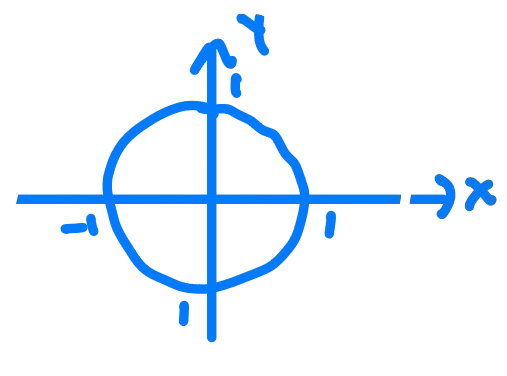
\includegraphics[width=0.35\textwidth]{polar curve sketch a.png}
    \caption{The graph of \( r = 1 \).}
    \label{fig:circle_graph}
\end{figure}
\end{solutionbox}

\subsection*{(b) \( \theta = \dfrac{\pi}{4} \)}
\addcontentsline{toc}{subsection}{Straight Line}

\begin{solutionbox}
Here, \( \theta = \dfrac{\pi}{4} \), and \( r \) can take any value. 

This represents all points that lie along the line passing through the origin at an angle of \( \frac{\pi}{4} \) (or \( 45^\circ \)) with the positive \( x \)-axis. The graph is a \textbf{straight line} through the origin.

\begin{conceptbox}
    \textbf{\underline{Cartesian Conversion}} \\ 
    In polar coordinates:
    \[
    \tan(\theta) = \frac{y}{x}
    \]
    Substituting \( \theta = \frac{\pi}{4} \), we get:
    \[
    \tan\left(\frac{\pi}{4}\right) = 1 \quad \Rightarrow \quad y = x
    \]
    Thus, the Cartesian equation is \( y = x \).
\end{conceptbox}
\begin{figure}[H]
    \centering
    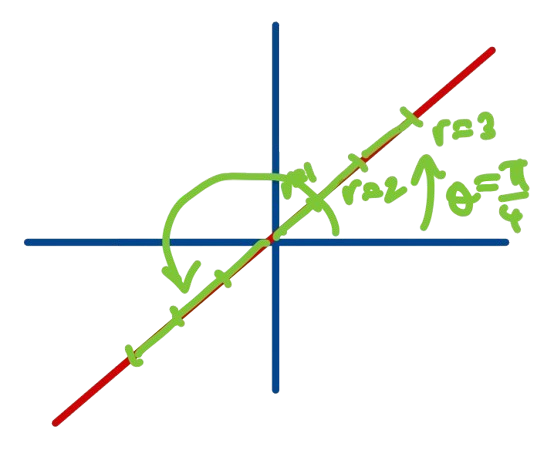
\includegraphics[width=0.8\textwidth]{polar curve sketch b.png}
    \caption{The graph of \( \theta = \frac{\pi}{4} \).}
    \label{fig:line_graph}
\end{figure}
\end{solutionbox}

\subsection*{(c) \( r = \theta, \quad \theta \geq 0 \)}
\addcontentsline{toc}{subsection}{Spiral}

\begin{solutionbox}
Here, \( r \) increases as \( \theta \) increases. This creates a \textbf{spiral} that starts at the origin and winds outward as \( \theta \) grows. 

\begin{conceptbox}
    \textbf{\underline{Table of Values}}
    \[
    \begin{array}{c|c}
    \theta & r \\
    \hline
    0 & 0 \\
    \frac{\pi}{6} & \frac{\pi}{6} \approx 0.52 \\
    \frac{\pi}{4} & \frac{\pi}{4} \approx 0.79 \\
    \frac{\pi}{3} & \frac{\pi}{3} \approx 1.05 \\
    \frac{\pi}{2} & \frac{\pi}{2} \approx 1.57 \\
    \end{array}
    \]
\end{conceptbox}
\begin{figure}[H]
    \centering
    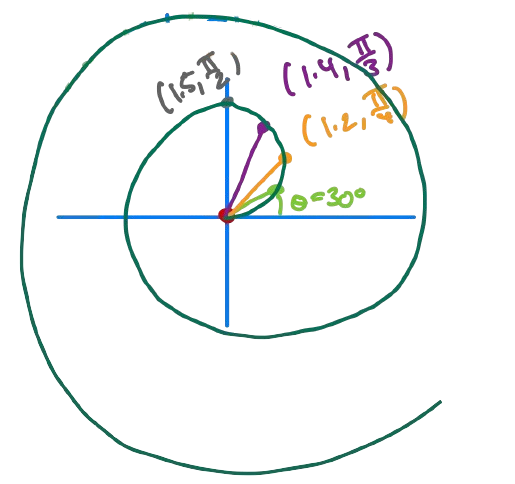
\includegraphics[width=0.75\textwidth]{polar curve sketch c.png}
    \caption{The graph of \( r = \theta \).}
    \label{fig:spiral_graph}
\end{figure}
\end{solutionbox}

\subsection*{(d) \( r = \sin(\theta) \)}
\addcontentsline{toc}{subsection}{Perfect-Circle Cardioid}

\begin{solutionbox}
Here, \( r = \sin(\theta) \). Since \( \sin(\theta) \) oscillates between \( 0 \) and \( 1 \), the graph forms a \textbf{cardioid} (which, in this case, is a perfect circle).

\begin{conceptbox}
    \textbf{\underline{Cartesian Conversion}} \\ 
    Using \( r^2 = x^2 + y^2 \) and \( r = \sin(\theta) \), we get:
    \[
    x^2 + y^2 = y \quad \Rightarrow \quad \left(x^2 + y^2\right) - y = 0
    \]
    Completing the square for \( y \):
    \[
    x^2 + \left(y - \frac{1}{2}\right)^2 = \frac{1}{4}
    \]
    This is a circle centred at \( (0, \frac{1}{2}) \) with radius \( \frac{1}{2} \).
\end{conceptbox}
\begin{figure}[H]
    \centering
    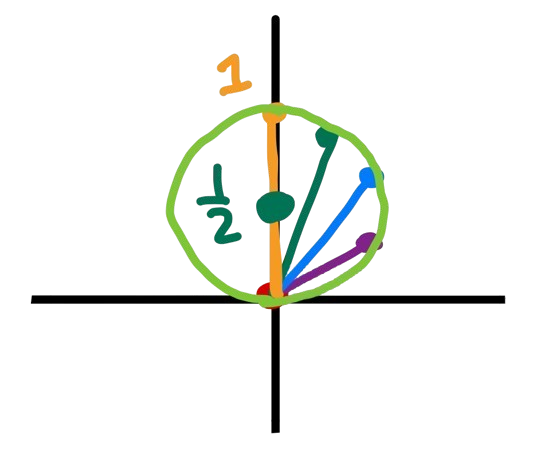
\includegraphics[width=0.7\textwidth]{polar curve sketch d.png}
    \caption{The graph of \( r = \sin(\theta) \).}
    \label{fig:cardioid_graph}
\end{figure}
\end{solutionbox}

\subsection*{(e) \( r = \cos(2\theta) \)}
\addcontentsline{toc}{subsection}{Four-Petaled Rose}

\begin{solutionbox}
The equation \( r = \cos(2\theta) \) represents a \textbf{four-petaled rose}. As \( \theta \) varies from \( 0 \) to \( 2\pi \), \( r \) oscillates between \( -1 \) and \( 1 \), creating the petals.

\begin{conceptbox}
    \textbf{\underline{Table of Values}} \\ 
    Evaluate \( r \) at critical angles:
    \[
    \begin{array}{c|ccccccccc}
    \theta & 0 & \frac{\pi}{4} & \frac{\pi}{2} & \frac{3\pi}{4} & \pi & \frac{5\pi}{4} & \frac{3\pi}{2} & \frac{7\pi}{4} & 2\pi \\
    \hline
    r & 1 & 0 & -1 & 0 & 1 & 0 & -1 & 0 & 1 \\
    \end{array}
    \]
    
    The curve is symmetric about the polar axis, with petals centered at \( \theta = 0, \frac{\pi}{2}, \pi, \frac{3\pi}{2} \).
\end{conceptbox}

\begin{figure}[H]
    \centering
    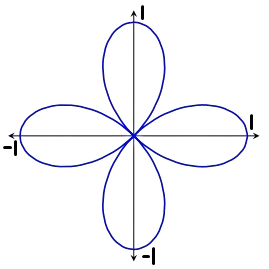
\includegraphics[width=0.35\textwidth]{polar curve sketch e.png}
    \caption{The graph of \( r = \cos(2\theta) \).}
    \label{fig:rose_graph}
\end{figure}
\end{solutionbox}

\section*{Homework Practice Problem: Polar Graph Sketching}
\begin{exercisebox}
    Try sketching the curve:
    \[
        r = \cos\theta
    \]
    under the same context as the previous questions.
    
    \begin{solutionbox}
    Here, \( r = \cos\theta \). Since \( \cos\theta \) oscillates between \( -1 \) and \( 1 \), the graph will form a \textbf{limacon} (which, in this case, simplifies to a standard circle) with an inner loop.
    
    \begin{conceptbox}
        \textbf{\underline{Table of Values}} \\
        To visualize the curve, create a table of key points:
        \[
        \begin{array}{c|ccccc}
        \theta & 0 & \frac{\pi}{3} & \frac{\pi}{2} & \frac{2\pi}{3} & \pi \\
        \hline
        r & 1 & \frac{1}{2} & 0 & -\frac{1}{2} & -1 \\
        \end{array}
        \]
        
        \begin{notebox}
            Plot the points in the table and connect them smoothly to form the graph. Note that for negative \( r \), the points are plotted in the opposite direction from the origin.
        \end{notebox}
    \end{conceptbox}
    \textit{...cont'd...}
    \end{solutionbox}
\end{exercisebox}
\begin{exercisebox}
    \begin{solutionbox}
        \textit{...cont'd...}
        \begin{conceptbox}
        \textbf{\underline{Cartesian Conversion}} \\

        To convert the polar equation \( r = \cos\theta \) into Cartesian form:
        \begin{enumerate}
            \item Recall the polar-to-Cartesian relationships:
            \[
            x = r \cos\theta \quad \text{and} \quad y = r \sin\theta.
            \]
            \item Substitute \( r = \cos\theta \) into \( x = r \cos\theta \):
            \[
            x = (\cos\theta)(\cos\theta) = \cos^2\theta.
            \]
            \item Using the Pythagorean identity \( \cos^2\theta + \sin^2\theta = 1 \), write \( \cos^2\theta \) as:
            \[
            \cos^2\theta = 1 - \sin^2\theta.
            \]
            \item Replace \( \sin^2\theta \) with \( \left(\dfrac{y}{r}\right)^2 \) since \( \sin\theta = \dfrac{y}{r} \):
            \[
            x = 1 - \left(\frac{y}{r}\right)^2.
            \]
            Multiply through by \( r^2 = x^2 + y^2 \) to eliminate \( r \):
            \[
            r^2x = r^2 - y^2 \quad \Rightarrow \quad (x^2 + y^2)x = x^2 + y^2 - y^2.
            \]
        \end{enumerate}

        After simplifying, we find:
        \[
        x^2 + y^2 = x.
        \]
        
        \textit{...cont'd...}
        \end{conceptbox}
    \end{solutionbox}
\end{exercisebox}
\begin{exercisebox}
    \begin{solutionbox}
        \textit{...cont'd...}
        \begin{conceptbox}
            \textbf{Completing the Square:} \\
            To identify the shape of this equation:
            \begin{enumerate}
                \item Isolate \( x^2 + x \):
                \[
                x^2 - x + y^2 = 0.
                \]
                \item Complete the square for \( x \):
                \[
                \left(x - \frac{1}{2}\right)^2 - \frac{1}{4} + y^2 = 0 \quad \Rightarrow \quad \left(x - \frac{1}{2}\right)^2 + y^2 = \frac{1}{4} = \left(\frac{1}{2}\right)^2.
                \]
            \end{enumerate}
    
            This represents a circle with:
            \begin{itemize}
                \item \textbf{Centre:} \( \left(\frac{1}{2}, 0\right) \),
                \item \textbf{Radius:} \( \frac{1}{2} \).
            \end{itemize}
        \end{conceptbox}
    
        \begin{figure}[H]
            \centering
            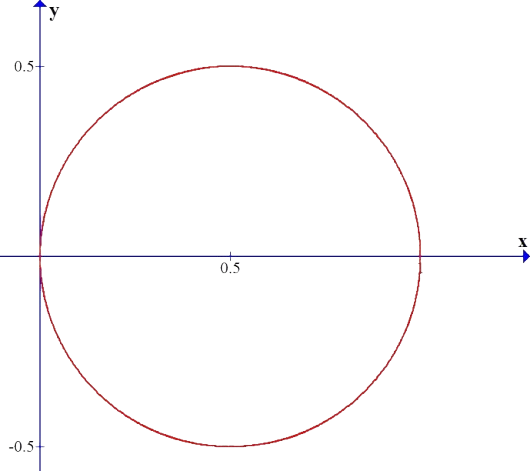
\includegraphics[width=0.55\textwidth]{hw practice question limacon.png}
            \caption{Graph of \( r = \cos\theta \), showing the limacon with an inner loop.}
            \label{fig:sample_image}
        \end{figure}
    \end{solutionbox}
\end{exercisebox}

\section*{Derivatives of Polar Curves and Their Applications}
\addcontentsline{toc}{section}{Derivatives of Polar Curves and Their Applications}

\subsection*{Tangents to Polar Curves: Finding Slopes and Key Conditions}
\addcontentsline{toc}{subsection}{Tangents to Polar Curves: Finding Slopes and Key Conditions}

\begin{theorembox}
\textbf{Tangent Slopes to Polar Curves} \\
Let an arbitrary polar curve be given by \( r = f(\theta) \), where \( r \) and \( \theta \) are related. The slope of the tangent line to the curve at a given point can be expressed as:

\[
    \dfrac{dy}{dx} = \dfrac{\dfrac{dy}{d\theta}}{\dfrac{dx}{d\theta}} = \dfrac{\dfrac{dr}{d\theta} \sin\theta + r \cos\theta}{\dfrac{dr}{d\theta} \cos\theta - r \sin\theta}.
\]

\textbf{\underline{Tangent Types:}}
\begin{itemize}
    \item \textbf{Horizontal Tangents:} Occurs when
    \[
        \frac{dy}{d\theta} = 0 \quad \text{and} \quad \frac{dx}{d\theta} \neq 0.
    \]
    \item \textbf{Vertical Tangents:} Occurs when
    \[
        \frac{dx}{d\theta} = 0 \quad \text{and} \quad \frac{dy}{d\theta} \neq 0.
    \]
    \item \textbf{Singular Points} (typically discarded in MAT232)\textbf{:} Occurs when both derivatives are zero\dots
    \[
        \frac{dy}{d\theta} = 0 \quad \text{and} \quad \frac{dx}{d\theta} = 0.
    \]
\end{itemize}
\textit{...cont'd...}
\end{theorembox}

\begin{theorembox}
    \textit{...cont'd...}
    
    \begin{conceptbox}
        \textbf{\underline{Derivation of the Tangent Slope}} \\
        
        To derive the formula for \( \dfrac{dy}{dx} \), we use the chain rule:
        \[
            \dfrac{dy}{dx} = \dfrac{\dfrac{dy}{d\theta}}{\dfrac{dx}{d\theta}}, \quad \text{where} \quad \dfrac{dx}{d\theta} \neq 0.
        \]
        
        Recall that \( r = f(\theta) \). First, compute the derivatives of \( x \) and \( y \) with respect to \( \theta \):
        \[
            \frac{dx}{d\theta} = \frac{d}{d\theta} \left( f(\theta) \cos\theta \right) = \frac{df(\theta)}{d\theta} \cos\theta - f(\theta) \sin\theta,
        \]
        \[
            \frac{dy}{d\theta} = \frac{d}{d\theta} \left( f(\theta) \sin\theta \right) = \frac{df(\theta)}{d\theta} \sin\theta + f(\theta) \cos\theta.
        \]
        
        Substitute these into the expression for \( \dfrac{dy}{dx} \):
        \[
            \frac{dy}{dx} = \dfrac{\dfrac{dy}{d\theta}}{\dfrac{dx}{d\theta}} = \dfrac{\dfrac{df(\theta)}{d\theta} \sin\theta + f(\theta) \cos\theta}{\dfrac{df(\theta)}{d\theta} \cos\theta - f(\theta) \sin\theta}.
        \]
        
        Finally, replace \( f(\theta) \) with \( r \), so we have the final expression:
        \LARGE
        \[
            \dfrac{dy}{dx} = \dfrac{\dfrac{dr}{d\theta} \sin\theta + r \cos\theta}{\dfrac{dr}{d\theta} \cos\theta - r \sin\theta}.
        \]
        \normalsize
        \end{conceptbox}
\end{theorembox}

\subsection*{Example: Finding the Vertical Tangent Angles on a Polar Curve}
\begin{examplebox}
Find the \textbf{vertical tangent} angles of the polar curve \( r = 1 - \cos\theta, \quad 0 \leq \theta \leq \pi \).

\begin{solutionbox}
We aim to determine the angles \( \theta \) where the polar curve has vertical tangents. This occurs when \( \dfrac{dx}{d\theta} = 0 \), provided \( \dfrac{dy}{d\theta} \neq 0 \).

\subsection*{Step 1: Compute \( \dfrac{dy}{dx} \)}
The derivative of a polar curve is given by:
\[
    \dfrac{dy}{dx} = \dfrac{\dfrac{dy}{d\theta}}{\dfrac{dx}{d\theta}} = 
    \dfrac{\dfrac{dr}{d\theta}\sin\theta + r\cos\theta}{\dfrac{dr}{d\theta}\cos\theta - r\sin\theta}.
\]

Given \( r = 1 - \cos\theta \), compute \( \dfrac{dr}{d\theta} \):
\[
    \dfrac{dr}{d\theta} = \sin\theta.
\]

Substitute \( r = 1 - \cos\theta \) and \( \dfrac{dr}{d\theta} = \sin\theta \) into the formula for \( \dfrac{dy}{dx} \):
\[
    \dfrac{dy}{dx} = 
    \dfrac{\sin\theta\sin\theta + (1 - \cos\theta)\cos\theta}{\sin\theta\cos\theta - (1 - \cos\theta)\sin\theta}.
\]

Simplify the numerator and denominator:
\[
    \dfrac{dy}{dx} = 
    \dfrac{\sin^2\theta - \cos^2\theta + \cos\theta}{\sin\theta(2\cos\theta - 1)}.
\]

\subsection*{Step 2: Condition for Vertical Tangents}
Vertical tangents occur when:
\[
    \dfrac{dx}{d\theta} = \sin\theta(2\cos\theta - 1) = 0,
\]
provided \( \dfrac{dy}{d\theta} \neq 0 \).
\end{solutionbox}
\textit{...cont'd...}
\end{examplebox}

\begin{examplebox}
    \textit{...cont'd...}
    \begin{solutionbox}
        Solve \( \dfrac{dx}{d\theta} = 0 \):
        \[
            \sin\theta = 0 \quad \text{or} \quad 2\cos\theta - 1 = 0.
        \]
        
        1. When \( \sin\theta = 0 \):
           \[
               \theta \in \{ 0, \pi \} \quad \text{(within \( 0 \leq \theta \leq \pi \))}.
           \]
        
        2. When \( 2\cos\theta - 1 = 0 \):
           \[
               \cos\theta = \dfrac{1}{2} \quad \Rightarrow \quad \theta = \dfrac{\pi}{3}.
           \]
        
        The candidates for vertical tangents are:
        \[
            \theta \in \{ 0, \dfrac{\pi}{3}, \pi \}.
        \]
        
        \subsection*{Step 3: Verify Each Candidate}
        To confirm vertical tangents, check \( \dfrac{dy}{dx} \neq 0 \) at these angles:
        \begin{itemize}
            \item For \( \theta = 0 \):
            \[
                \dfrac{dx}{d\theta} = \sin(0)(2\cos(0) - 1) = 0, \quad 
                \dfrac{dy}{d\theta} = 0 \quad \Rightarrow \text{discard}.
            \]
            \item For \( \theta = \dfrac{\pi}{3} \):
            \[
                \dfrac{dx}{d\theta} \neq 0 \quad \Rightarrow \text{valid vertical tangent}.
            \]
            \item For \( \theta = \pi \):
            \[
                \dfrac{dx}{d\theta} = \sin(\pi)(2\cos(\pi) - 1) = 0, \quad 
                \dfrac{dy}{d\theta} \neq 0 \quad \Rightarrow \text{valid vertical tangent}.
            \]
        \end{itemize}
        
        \begin{answerbox}
        The vertical tangents are located at:
        \[
            \theta = \dfrac{\pi}{3} \quad \text{and} \quad \theta = \pi.
        \]
        \end{answerbox}
    \end{solutionbox}
    \textit{...cont'd...}
\end{examplebox}

\begin{examplebox}
    \textit{...cont'd...}
    \begin{figure}[H]
        \centering
        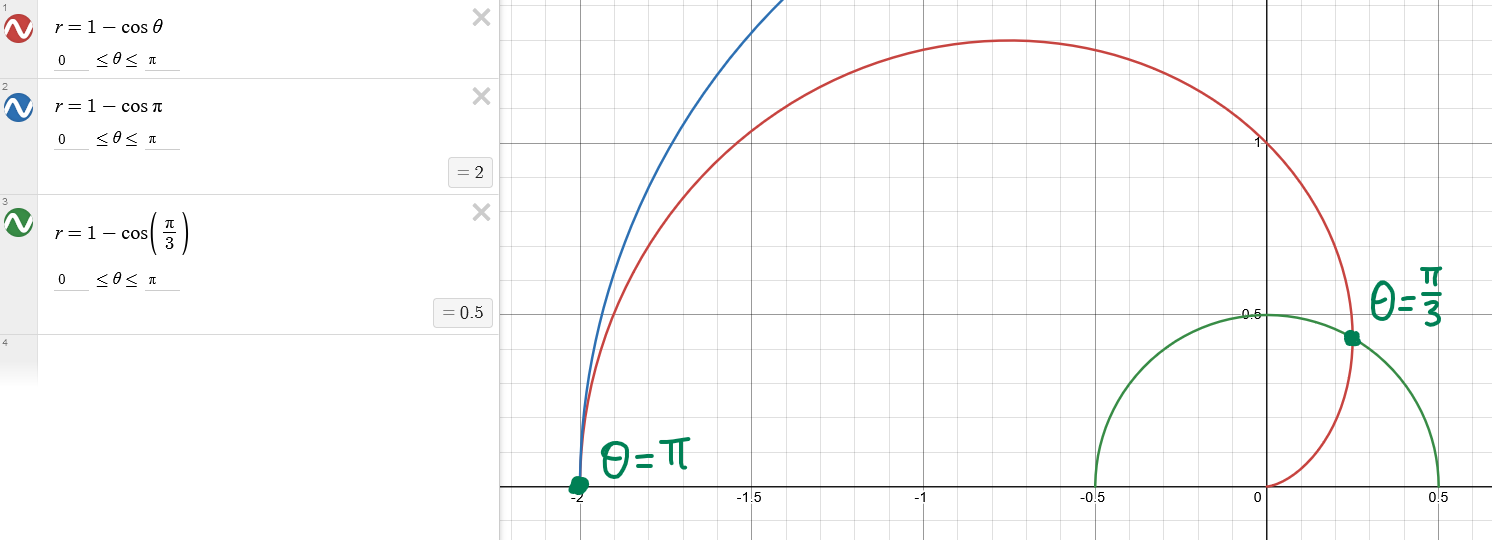
\includegraphics[width=1\textwidth]{demo for 1 - cos(theta).png}
        \caption{Illustration of vertical tangent positions for \( r = 1 - \cos\theta \).}
        \label{fig:vertical_tangents}
    \end{figure}
\end{examplebox}

\section*{Equations of Circles in the Cartesian Plane}
\addcontentsline{toc}{section}{Equations of Circles in the Cartesian Plane}

\begin{theorembox}
    The equations below describe the geometry of a circle in the Cartesian plane:
    
    \begin{itemize}
        \item \textbf{Standard Circle:} A circle centered at the origin \((0, 0)\) with radius \(r\) is given by:
        \[
            x^2 + y^2 = r^2.
        \]
        This equation represents a circle with radius \(r\), where every point on the circle is exactly \(r\) units away from the origin.

        \item \textbf{General Circle:} A circle centered at \((h, k)\) with radius \(r\) is described by:
        \[
            (x - h)^2 + (y - k)^2 = r^2.
        \]
        This equation represents a circle with center at the point \((h, k)\) and radius \(r\). Each point on this circle is at a distance of \(r\) from the center \((h, k)\).
    \end{itemize}
    
    \begin{figure}[H]
        \centering
        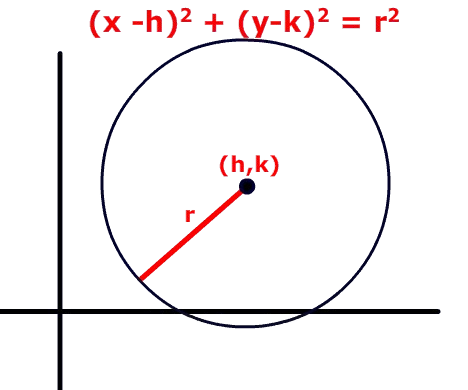
\includegraphics[width=0.43\textwidth]{equation of a circle.png}
        \caption{Graphical representation of a circle in the Cartesian plane.}
        \label{fig:sample_image1}
    \end{figure}

    \begin{notebox}
        \begin{itemize}
            \item In the case of the \textbf{standard circle}, the center of the circle is at the origin \((0, 0)\), making the equation simple as \(x^2 + y^2 = r^2\).
            \item For the \textbf{general circle}, the center is at \((h, k)\), and the equation adjusts accordingly.
            \begin{enumerate}
                \item[\labelitemi] The terms \((x - h)\) and \((y - k)\) shift the circle to the new center.
            \end{enumerate}
        \end{itemize}
    \end{notebox}
\end{theorembox}

\subsection*{Exercise: Sketching a Circle Curve}
\addcontentsline{toc}{subsection}{Exercise: Sketching a Circle Curve}
\begin{exercisebox}
    \textbf{Example:} Sketch the curve described by the equation:
    \[
        x^2 + y^2 - 2x = 10.
    \]
    
    \begin{solutionbox}
    To sketch the curve, we need to rewrite the given equation in the standard form of a circle. We will do this by completing the square for the \(x\)-terms.

    \subsubsection*{Step 1: Group \(x\)-terms and prepare to complete the square}
    First, we want to isolate the terms involving \(x\) on one side of the equation:
    \[
        x^2 - 2x + y^2 = 10.
    \]
    Notice that the \(y\)-terms are already in a simple form, and we will handle the \(x\)-terms separately.

    \subsubsection*{Step 2: Complete the square for \(x\)}
    To complete the square, we focus on the expression \(x^2 - 2x\):
    \begin{itemize}
        \item Divide the coefficient of \(x\) by 2: 
        \[
            -\frac{2}{2} = -1.
        \]
        \item Then square the result:
        \[
            (-1)^2 = 1.
        \]
        \item Now, add and subtract this square, \(1\), to the equation to maintain equality:
        \[
            x^2 - 2x + 1 + y^2 = 10 + 1.
        \]
        This does not change the equation, but it allows us to rewrite the \(x\)-terms as a perfect square.
    \end{itemize}
    \end{solutionbox}
    \textit{...cont'd...}
\end{exercisebox}

\begin{exercisebox}
    \textit{...cont'd...}
    \begin{solutionbox}
        \subsubsection*{Step 3: Rewrite as a perfect square}
        Now, we can express the \(x\)-terms as a perfect square:
        \[
            (x - 1)^2 + y^2 = 11.
        \]
        This equation is now in the standard form of a circle, where:
        \[
            (x - h)^2 + (y - k)^2 = r^2,
        \]
        with \(h = 1\), \(k = 0\), and \(r^2 = 11\).
    
        \subsubsection*{Final Form and Interpretation}
        The equation \((x - 1)^2 + y^2 = 11\) represents a circle. From the standard form, we can directly read the center and radius:
        \begin{itemize}
            \item The center of the circle is \((h, k) = (1, 0)\).
            \item The radius of the circle is \(r = \sqrt{11}\), as the radius is the square root of \(r^2\).
        \end{itemize}
        
        \begin{tipbox}
        The circle is centered at \((1, 0)\) and has a radius of \(\sqrt{11}\).
        \end{tipbox}

        \begin{figure}[H]
            \centering
            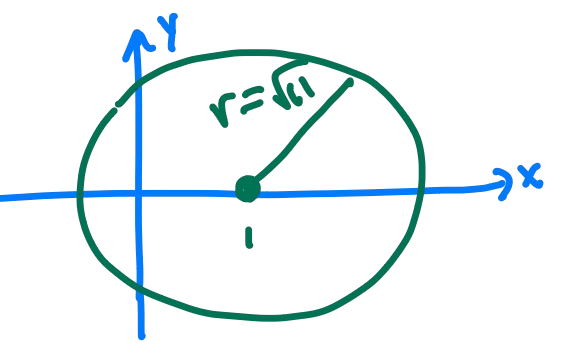
\includegraphics[width=.5\textwidth]{equation of a circle example question.png}
            \caption{Illustration of the circle with center \( (1, 0) \) and radius \( \sqrt{11} \).}
            \label{fig:circle_example}
        \end{figure}        
    \end{solutionbox}
\end{exercisebox}

\end{document}
